%https://www.integral-domain.org/lwilliams/Resources/TikzImg/isopaper.tex
\documentclass[tikz]{standalone}

\begin{document} 
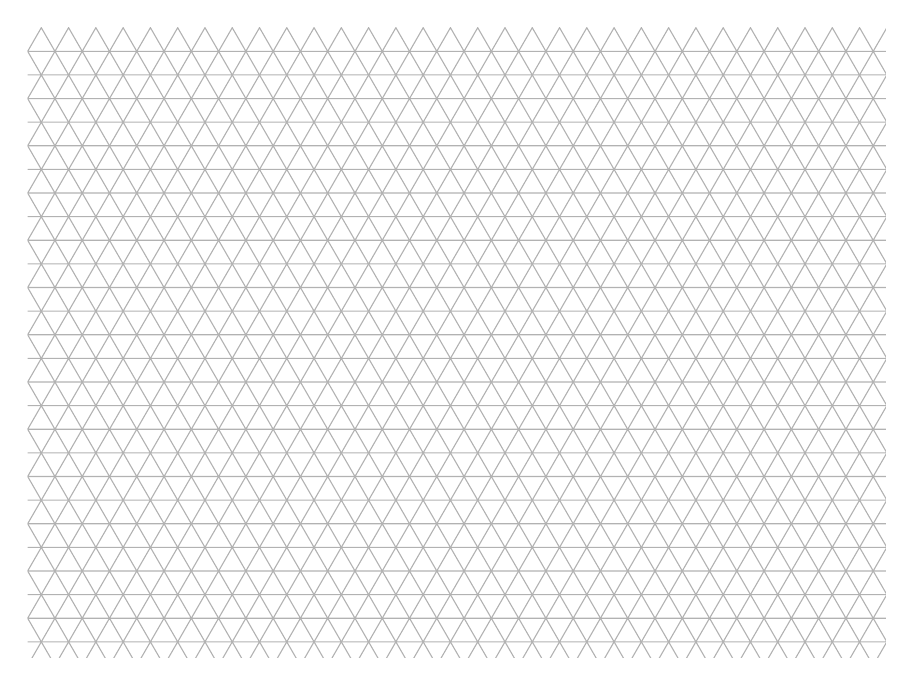
\begin{tikzpicture}

% paper size:
\pgfmathsetmacro\pwidth{10.9};
\pgfmathsetmacro\pheight{8};
% triangle outer radius:
\pgfmathsetmacro\R{0.2};
 
\clip(0,0) rectangle (\pwidth,\pheight); 


\pgfmathsetmacro\a{1.732*\R}
\pgfmathsetmacro\ncols{\pwidth/\a}
\pgfmathsetmacro\nrows{\pheight/(\R*1.5)}

\foreach \col in {0,1,2,...,\ncols}{
  \foreach \row in {0,1,2,...,\nrows} {
    \ifodd\row
      \begin{scope}[xshift=\a*\col cm, yshift=1.5*\R*\row cm]
       \draw[thin, black!30] (90:\R)--(210:\R)--(330:\R)--cycle;
      \end{scope}
    \else 
      \begin{scope}[xshift=\a*\col cm+0.5*\a cm, yshift=1.5*\R*\row cm]
       \draw[thin, black!30] (90:\R)--(210:\R)--(330:\R)--cycle;
    \end{scope}
    \fi 
  }
}
 

\end{tikzpicture} 
\end{document}
